\begin{description}
\item[H1:] Participants performed on average 20.62\% better using the predictive display versus no predictive display, t(56)=4.80, p$<$.001, d=0.904. H1, that a simple predictor display based on image transformation can increase the operator performance, is therefore verified.

\item[H2:] The participants did not reported any significant difference in the mental, physical or temporal demand using the predictive display. H2, that a simple predictor display based on image transformation will decrease the operator's subjective workload, has to be rejected. 
\end{description}
\vspace{-5mm}
\section{Performance}

\figref{performanceNorm} shows the normalized number of hits in 90 seconds (score), for each display type and all N=57 participants. \textit{Delay} refers to the \textit{added} delay, which means that "No delay" translates to the inherent system delay of $250 ms$. The numerical values are reported in Table \ref{score}. The statistical significance and effect size between conditions can be seen in Table \ref{score2}.

\begin{figure}[h!]
    \centering
    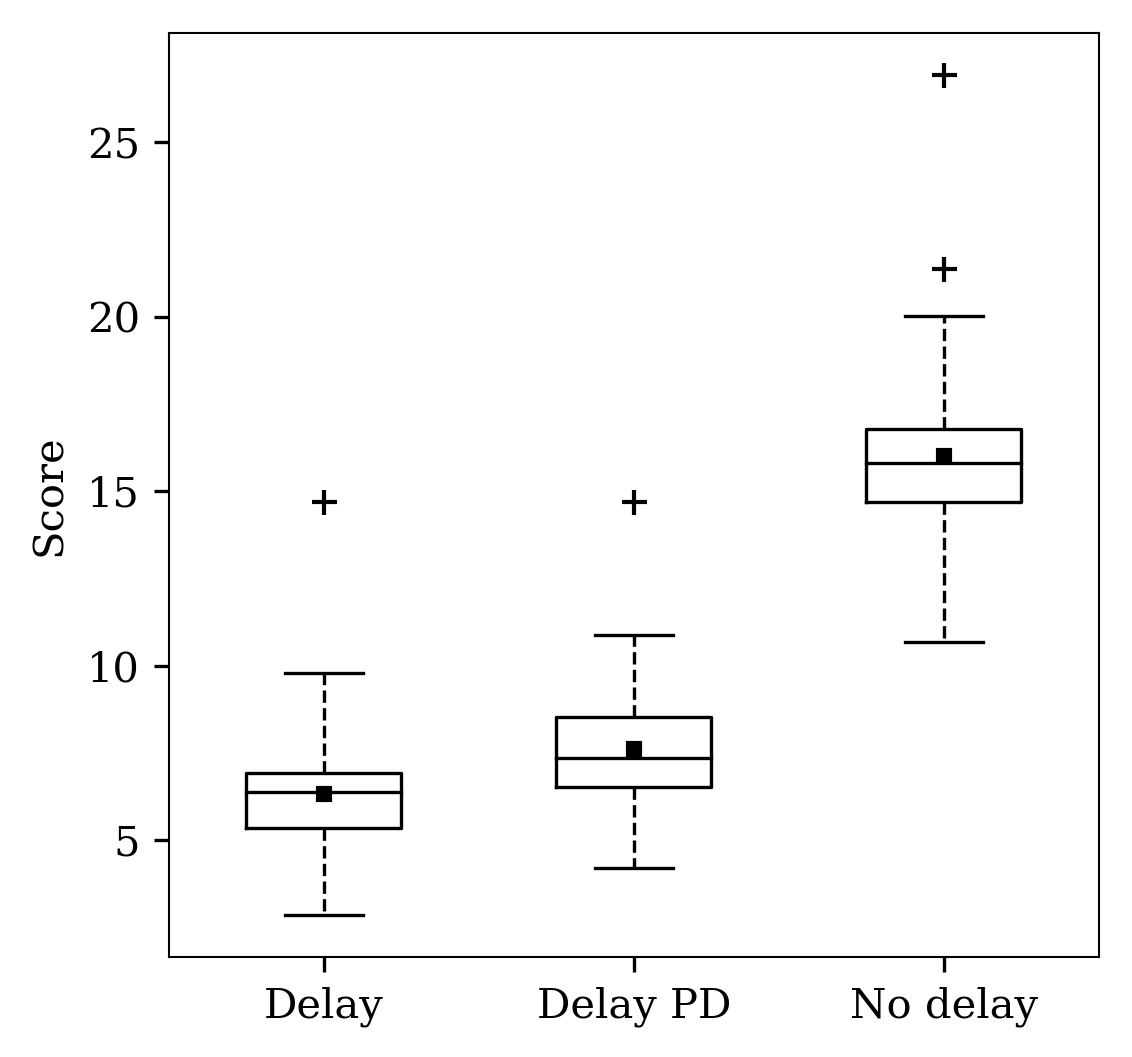
\includegraphics[scale=0.85]{performance_norm}
    \caption{Normalized score all participants, N=57.}
    \label{performanceNorm}
	\vspace{-0.2cm}
\end{figure}

Those who play games weekly or more were defined as \emph{gamers}. They performed on average 30.13\% better, while non-gamers only saw a 16.91\% performance increase with the PD. This difference is illustrated in \figref{gamer_performance}.

% Please add the following required packages to your document preamble:
% \usepackage{booktabs}
\begin{table}[]
\small
\centering
\caption{Normalized mean scores and standard deviation (SD).}
\label{score}
\begin{tabularx}{\textwidth}{@{}XXXXX@{}}
\toprule
Differentiation & Group       & Display  & Score & SD \\ \midrule
None            & All N=57    & Delay    & 6.24  & 1.39               \\
                &             & Delay PD & 7.52  & 1.43               \\
                &             & No delay & 15.87 & 1.99               \\ \addlinespace
Gender          & Male n=38   & Delay    & 6.65  & 1.25               \\
                &             & Delay PD & 7.95  & 1.43               \\
                &             & No delay & 17.30 & 1.71               \\ \addlinespace
                & Female n=19 & Delay    & 5.39  & 1.49               \\
                &             & Delay PD & 6.61  & 1.35               \\
                &             & No delay & 13.10 & 2.17               \\ \addlinespace
Gaming          & Daily n=2   & Delay    & 7.92  & 0.37               \\
                &             & Delay PD & 10.21 & 1.40               \\
                &             & No delay & 18.36 & 1.77               \\ \addlinespace
                & Weekly n=15 & Delay    & 6.27  & 1.22               \\
                &             & Delay PD & 8.17  & 1.51               \\
                &             & No delay & 17.62 & 2.04               \\ \addlinespace
                & Monthly n=8 & Delay    & 7.05  & 1.32               \\
                &             & Delay PD & 7.77  & 0.64               \\
                &             & No delay & 17.68 & 0.95               \\ \addlinespace
                & Yearly n=17 & Delay    & 6.65  & 1.26               \\
                &             & Delay PD & 7.66  & 1.73               \\
                &             & No delay & 15.98 & 2.25               \\ \addlinespace
                & Never n=15  & Delay    & 5.06  & 1.46               \\
                &             & Delay PD & 6.21  & 1.16               \\
                &             & No delay & 12.73 & 1.79               \\ \bottomrule
\end{tabularx}
\end{table}
% Please add the following required packages to your document preamble:
% \usepackage{booktabs}
\begin{table}[]
\centering
\caption{Paired samples t-test and Cohen's d effect size}
\label{score2}
\begin{tabularx}{\textwidth}{@{}llYYYY@{}}
\toprule
\multicolumn{2}{c}{Pair} & \multicolumn{3}{c}{t-test for Equality of Means} &       \\ \cmidrule(lr){3-5}
\multicolumn{2}{l}{}     & t                  & df             & p                   & d     \\ \midrule
Delay       & Delay PD   & 4.82               & 56             & $<$.001             & 0.735 \\
Delay       & No delay   & 23.04              & 56             & $<$.001             & 4.413 \\
Delay PD    & No delay   & 19.52              & 56             & $<$.001             & 3.861 \\ \bottomrule
\end{tabularx}
\end{table}

\begin{figure}[h!]
    \centering
    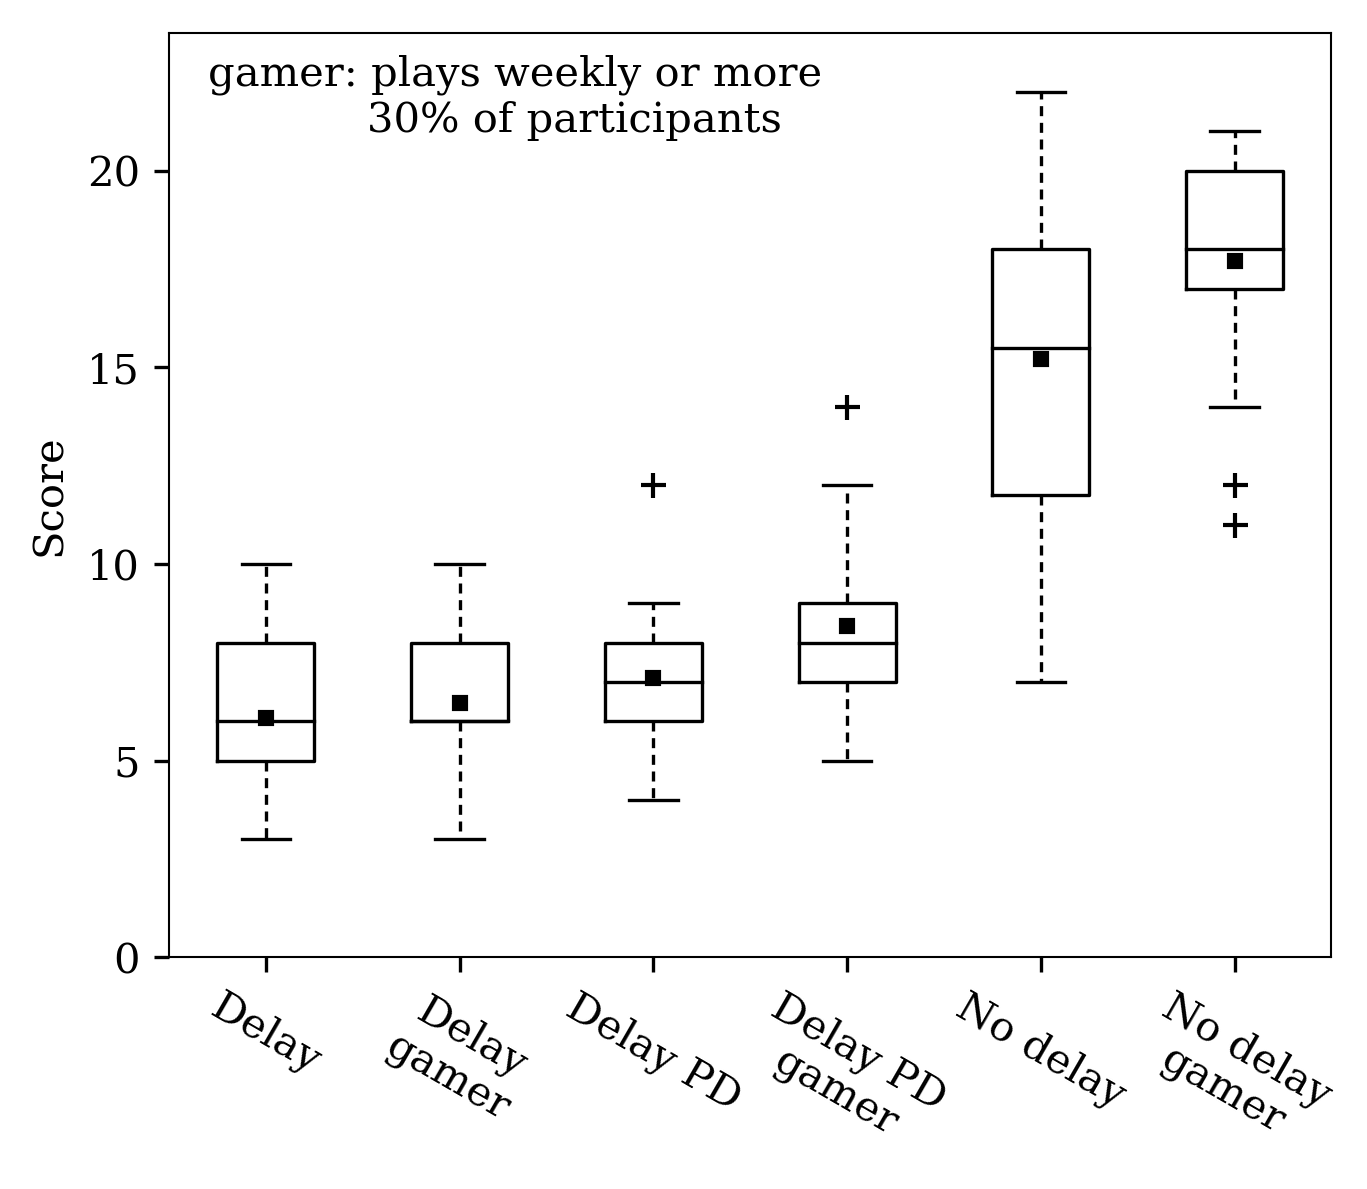
\includegraphics[scale=0.85]{gamer_performance}
    \caption{Performance of gamers n=17, versus non-gamers n=40.}
    \label{gamer_performance}
\end{figure}

\clearpage
\section{Task load index}

\figref{tlx} shows the reported NASA TLX scores. The height of the bar describes the mean value while the whiskers shows the SD. Numerical values are reported in Table \ref{tlx_values}.

There are no big differences between condition one and two. The only significant differences between those two conditions can be found in the \emph{performance}, t(56)=3.24, p=0.002, d=0.360 and \emph{frustration}, t(56)=2.15, p=0.036, d=0.271 metric. This means that the subjects felt less frustration and evaluated their performance as better when using the predictive display.

\begin{figure}[h!]
    \centering
    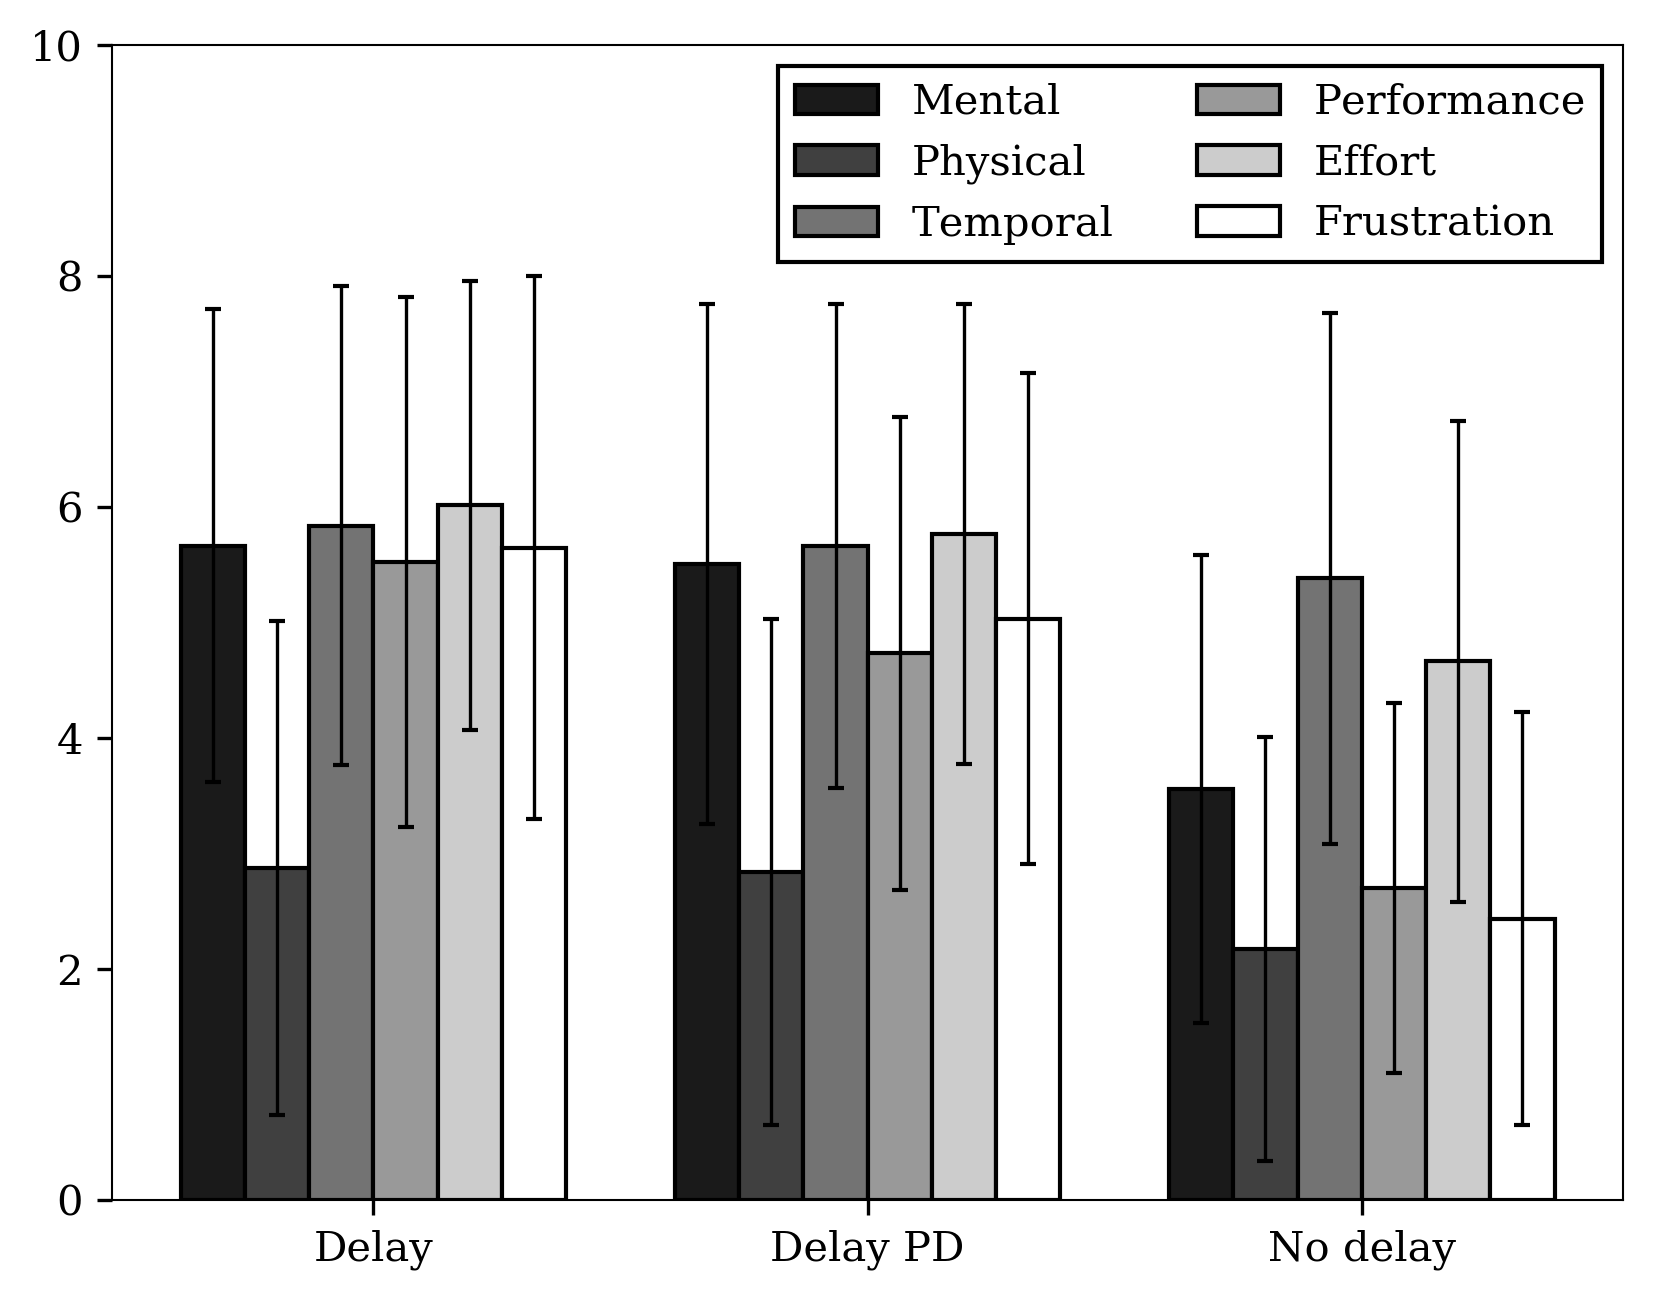
\includegraphics[scale=0.85]{nasa_tlx_bar}
    \caption{NASA TLX (task load index) results for each display type, N=57. Lower is better.}
    \label{tlx}
\end{figure}

% Please add the following required packages to your document preamble:
% \usepackage{booktabs}
\begin{table}[]
\small
\centering
\caption{Rated NASA TLX values and standard deviation (SD), N=57. Lower is better.}
\label{tlx_values}
\begin{tabularx}{\textwidth}{@{}XXXX@{}}
\toprule
Metric      & Display  & Rated value & SD \\ \midrule
Mental      & Delay    & 5.67        & 2.05               \\
            & Delay PD & 5.51        & 2.25               \\
            & No delay & 3.56        & 2.03               \\\addlinespace
Physical    & Delay    & 2.88        & 2.14               \\
            & Delay PD & 2.84        & 2.19               \\
            & No delay & 2.18        & 1.84               \\\addlinespace
Temporal    & Delay    & 5.84        & 2.08               \\
            & Delay PD & 5.67        & 2.10               \\
            & No delay & 5.39        & 2.30               \\\addlinespace
Performance & Delay    & 5.53        & 2.29               \\
            & Delay PD & 4.74        & 2.05               \\
            & No delay & 2.70        & 1.60               \\\addlinespace
Effort      & Delay    & 6.02        & 1.94               \\
            & Delay PD & 5.77        & 1.99               \\
            & No delay & 4.67        & 2.08               \\\addlinespace
Frustration & Delay    & 5.65        & 2.35               \\
            & Delay PD & 5.04        & 2.13               \\
            & No delay & 2.44        & 1.79               \\ \bottomrule
\end{tabularx}
\end{table}
\clearpage
\section{Subjective delay}

\figref{subjective_delay_norm} shows the normalized reported total delay in seconds for the three conditions. The participants reported a 11\% decrease in subjective latency using the predictive display versus the normal display with the same latency. This results is however not significant, t(56)=1.40, p=0.167, d=0.356.


\begin{figure}[h!]
    \centering
    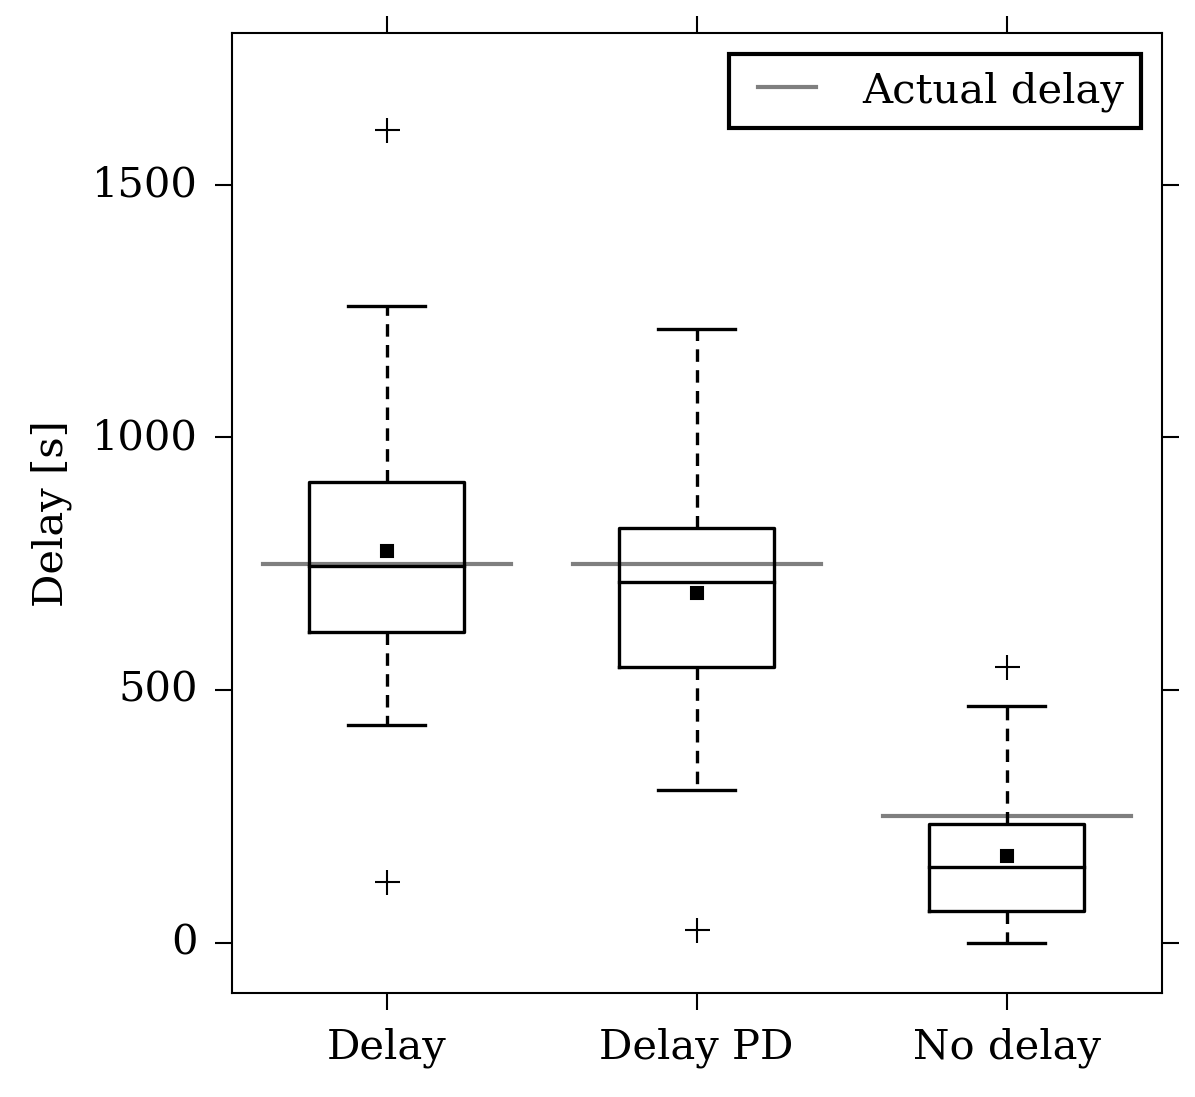
\includegraphics[scale=0.85]{subjective_delay_norm}
    \caption{Normalized reported subjective latency in seconds.}
    \label{subjective_delay_norm}
\end{figure}

\section{Key presses}

\figref{keypresses} shows the number of key presses performed during the 90 seconds of task time for each display type. With a low latency, participants are in a greater degree trying to continuously maneuver the ROV.

\begin{figure}[h!]
    \centering
    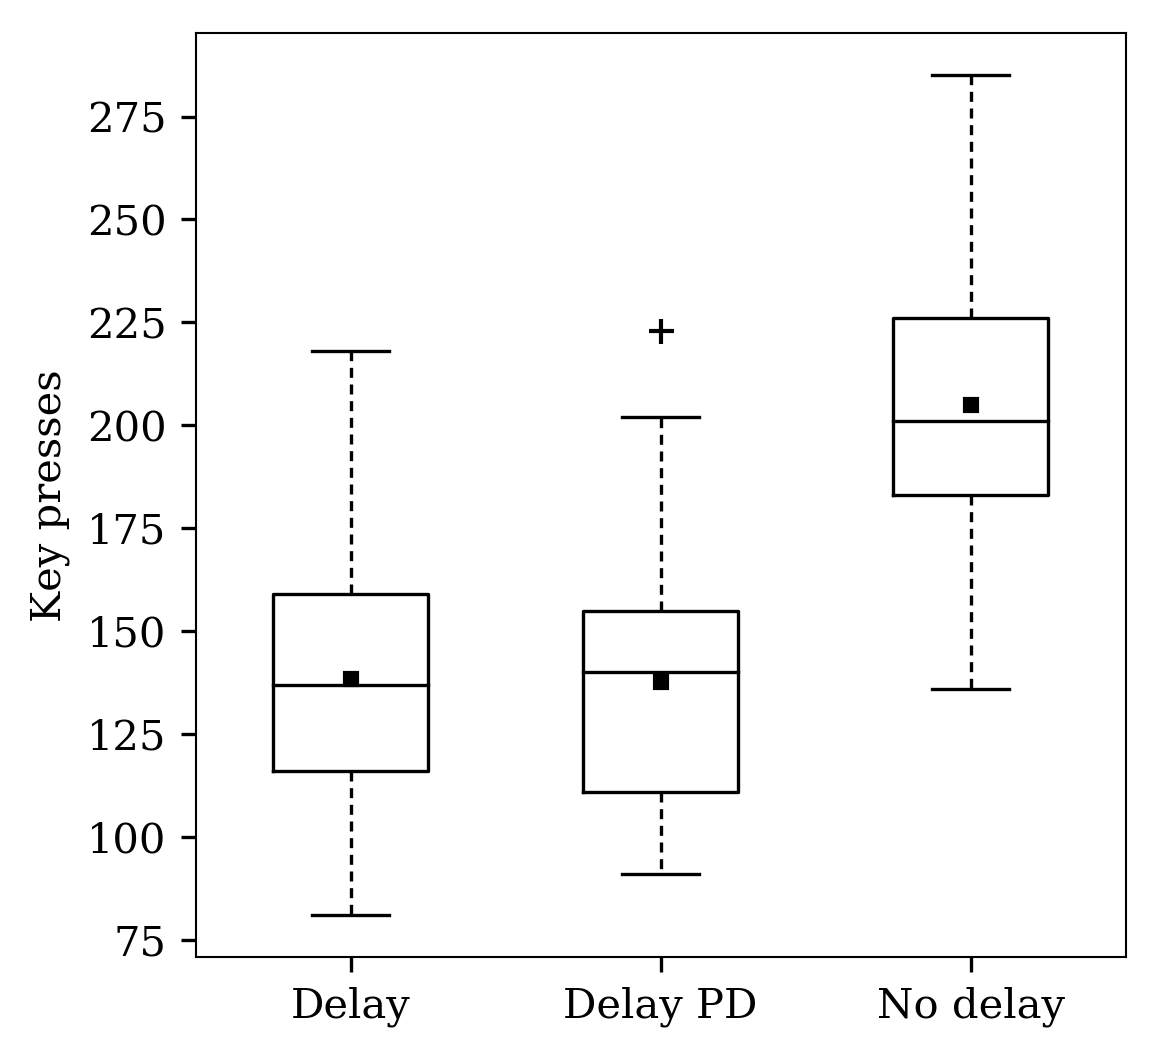
\includegraphics[scale=0.85]{keypresses}
    \caption{The number of key presses performed during 90 seconds.}
    \label{keypresses}
\end{figure}

